\documentclass[preprint,10pt]{elsarticle}
\usepackage[margin=2.5cm]{geometry}
\usepackage{graphicx} % Required for inserting images
\usepackage{amsmath} % for math
\usepackage{amssymb} % for symbols
\usepackage{hyperref} % for hyperlinks
\usepackage{fancyhdr} % for headers
\usepackage{geometry} % to change the page dimensions
\usepackage{multicol}
\usepackage{url} % for URLs
\usepackage{multirow}
\usepackage{biblatex}
\addbibresource{ref.bib}
\usepackage{float}
\usepackage{biblatex}
\usepackage{lscape}
\usepackage{pdflscape}
\usepackage{tabularx}

%\usepackage[style=authoryear,sorting=ynt]{biblatex}
\makeatletter
\def\ps@pprintTitle{%
 \let\@oddhead\@empty
 \let\@evenhead\@empty
 \let\@oddfoot\@empty
 \let\@evenfoot\@empty
}
\makeatother




\title{\Large\textbf{Tight Dynamic Problem Lower Bounds from Generalized BMM and OMv\textsuperscript{*}}}
\author[]{
\begin{tabular}{lllclllllllllllclll}
\begin{tabular}[c]{@{}c@{}}\textbf{Ce Jin\textsuperscript{\dag}}\\ cejin@mit.edu\\ MIT\\ Cambridge, MA, USA\end{tabular} &  &  &  &  &  &  &  &  &  &  &  & \begin{tabular}[c]{@{}c@{}}\textbf{Yinzhan Xu\textsuperscript{\ddag}}\\ xyzhan@mit.edu\\ MIT\\ Cambridge, MA, USA\end{tabular} &  &  & 
\end{tabular}
}

\begin{document}

\maketitle


\begin{multicols}{2}

 \textbf{Abstract}\\
  Popular fine-grained hypotheses have been successful in proving conditional lower bounds for many dynamic problems. Two of the most widely applicable hypotheses in this context are the \emph{combinatorial Boolean Matrix Multiplication (BMM) hypothesis}  and the closely-related \emph{Online Matrix Vector Multiplication (OMv) hypothesis}. The main theme of this paper is using $k$-dimensional generalizations of these two hypotheses to prove new \emph{tight} conditional lower bounds for dynamic problems.

The \emph{combinatorial $k$-Clique hypothesis}, which is a standard hypothesis in the literature, naturally generalizes the combinatorial BMM hypothesis. In this paper, we prove tight lower bounds for several dynamic problems under the combinatorial $k$-Clique hypothesis. For instance, we show that.The \emph{Dynamic Range Mode} problem has no combinatorial algorithms with $\mathrm{poly}(n)$ pre-processing time, $O(n^{2/3-\epsilon})$ update time and $O(n^{2/3-\epsilon})$ query time for any $\epsilon > 0$, matching the known upper bounds for this problem. Previous lower bounds only ruled out  algorithms with $O(n^{1/2-\epsilon})$ update and query time under the OMv hypothesis.
      The \emph{Dynamic Subgraph Connectivity} problem on undirected graphs with $m$ edges has no combinatorial algorithms with $\mathrm{poly}(m)$ pre-processing time, $O(m^{2/3-\epsilon})$ update time and $O(m^{1-\epsilon})$ query time for $\epsilon > 0$, matching the upper bound given by  Chan, P{\u{a}}tra{\c{s}}cu,
      and Roditty~[SICOMP'11], and improving the previous update time lower bound (based on OMv) with 
 \begin{minipage}[t]{\linewidth}
\footnote{
{The full version of this paper is available at \href{https://arxiv.org/abs/2202.11250}{https://arxiv.org/abs/2202.11250}.}\\
{Supported by NSF Grant CCF-2129139.}\\
{Supported by NSF Grant CCF-2129139.}


    
\includegraphics[scale=0.2]{image.png} 
    \\
    This work is licensed under a Creative Commons Attribution 4.0 International License.\\
    \textit{STOC '22, June 20--24, 2022, Rome, Italy}\\
    \copyright 2022 Copyright held by the owner/author(s).\\
    ACM ISBN 978-1-4503-9264-8/22/06.\\
    \href{https://doi.org/10.1145/3519935.3520036}{https://doi.org/10.1145/3519935.3520036}
}
\end{minipage}
      exponent $1/2$Other examples include tight combinatorial lower bounds for \emph{Dynamic 2D Orthogonal Range Color Counting}, \emph{Dynamic 2-Pattern Document Retrieval}, and \emph{Dynamic Range Mode} in higher dimensions.
	
Furthermore, we propose the OuMv$_k$ hypothesis as a natural generalization of the OMv hypothesis. Under this hypothesis, we prove tight lower bounds for various dynamic problems. For instance, we show that The \emph{Dynamic Skyline Points Counting} problem in $(2k-1)$-dimensional space has no algorithm with $\mathrm{poly}(n)$ pre-processing time and $O(n^{1-1/k-\epsilon})$ update and query time for $\epsilon > 0$, even 
Other examples include tight conditional lower bounds for (semi-online) Dynamic Klee's measure for unit cubes, and high-dimensional generalizations of Erickson’s problem and Langerman’s problem.  \\

  \textbf{CCS CONCEPTS}
  \begin{itemize}
      \item Theory of computation → Data structures design and anal-ysis.
  \end{itemize} 
  
  \textbf{KEYWORDS}\\
  fine-grained complexity, dynamic data structures\\
  
  \textbf{\emph{ACM Reference Format}}:Ce Jin and Yinzhan Xu. 2022. Tight Dynamic Problem Lower Bounds fromGeneralized BMM and OMv. In Proceedings of the 54th Annual ACM SIGACTSymposium on Theory of Computing (STOC ’22), June 20ś24, 2022, Rome, Italy.ACM, New York, NY, USA, 14 pages. \url{https://doi.org/10.1145/3519935.3520036}\\

  \section{INTRODUCTION}
  Dynamic data structure problems involve maintaining datasets (like graphs or sequences) that undergo small updates while supporting efficient queries. These problems are motivated by real-world applications, such as social network graphs and real-time systems, where data frequently changes. Despite progress, many dynamic problems, such as directed graph reachability, still have only slow, polynomial-time solutions. Researchers aim to establish lower bounds for such problems through fine-grained complexity, using hypotheses like combinatorial Boolean Matrix Multiplication (BMM) and Online Matrix-Vector Multiplication (OMv) to prove conditional lower bounds for dynamic problem hardness.\\



  \textbf{Hypothesis 1.1}\label{1.1} (Combinatorial k-Clique Hypothesis). There is 
no $O(n^{k-\epsilon})$ time combinatorial algorithm for k-Clique Detection on
n-vertex graphs, for any $\epsilon > 0$.\\
\textbf{Definition 1.2}\label{1.2} 2 (OuMv$_k$ Problem). During pre-processing we are
given a subset $M\subseteq [n]^{k.3}$ Then we receive online queries each
specifying k sets $U^{(1)},U^{(2)},...,U^{(k)} \subseteq [n]$, and we need to answer
whether $U^{(1)},U^{(2)},...,U^{(k)}$ has a non-empty intersection
with M.

\textbf{Hypothesis 1.3}\label{1.3}(OuMv$_k$ Hypothesis). There is no algorithm for
the OuMv$_k$ problem with n queries in $O(n^{1+k-\epsilon})$ total time (preprocessing time plus total query time) for any $\epsilon > 0$.

\textbf{Hypothesis 1.4}\label{1.4} There is no algorithm for the OuMv$_k$ problem with
poly(n) pre-processing time and $O(n^{\gamma+\kappa-\epsilon})$ total query time for $n^{\gamma}$ queries, for any  $\gamma,\epsilon > 0.$

\subsection{\textbf{Our Contribution}}

    \textbf{Theorem 1.5.}\label{1.5} Assuming the combinatorial 4-Clique hypothesis,
there is no combinatorial data structure that solves Dynamic Range
Mode in poly(n) pre-processing time, $O(n^{2/3-\epsilon})$ amortized query
time and  $O(n^{2/3-\epsilon})$ amortized update time for  $\epsilon>0$. The same lower
bound also holds for the Dynamic Range Minority problem.\\

Previous conditional lower bounds have ruled out algorithms for
SubConn with any of the following running times (for any $\epsilon > 0$):

   \begin{enumerate}
        \item (under 3SUM \cite{6979028}) $O(m^{4/3-\epsilon})$ pre-processing, $O(m^{a-\epsilon})$ update and $O(m^{2/3-a-\epsilon})$ query time, for any $a \in [fraq{1}{6},fraq{1}{3}]$.
\item (under OMv \cite{10.1145/2746539.2746609}) polynomial pre-processing, $O(m^{a-\epsilon})$  update and $O(m^{1-a-\epsilon})$ query time, for any $a \in (0, 1)$.

\item (under OMv \cite{10.1145/2746539.2746609}) polynomial pre-processing, $O(m^{1/2-\epsilon})$ update and $O(m^{1-\epsilon})$ query time.

\end{enumerate}

\textbf{Theorem 1.6}\label{1.6} Assuming the combinatorial 4-Clique hypothesis,
there is no combinatorial algorithm that solves st-SubConn in (m) pre-processing time, $O(m^{2/3-\epsilon})$ amortized update time, and $O(m^{1-\epsilon})$ amortized query time for $\epsilon > 0$.
We leave it as an open problem to either improve the 2/3 exponent in the update time using fast matrix multiplication or determine it’s impossible.

  \textbf{Problem 1}\label{prob 1} [Dynamic 2-Pattern Document Retrieval]. Given a list
of strings $S_1,....,S_D$ of total length $\sum_{i=1}^{D} |S_i| = n$, where each string is on or off, maintain a data structure that supports the following
operations:
\begin{itemize}
    \item Turn on or turn off a string;
    \item  Given a pair of strings $(T_1,T_2)$, count the number of i such that $S_i$ is on and contains both $T_1$ and $T_2$.
    \end{itemize}
            

We show (in the full paper) that this problem can be solved
by a combinatorial data structure with $O(n^{2/3})$ time per update
and $O(|T_1| + |T_2|+n^{2/3})$ time per query. Under the combinatorial 4-Clique hypothesis, this data structure is in fact optimal among combinatorial ones.\\






\textbf{Theorem 1.7}\label{1.7}Assuming the combinatorial $4$-Clique hypothesis, there is no combinatorial data structure that solves the Dynamic $2$-Pattern Document Retrieval problem in $(n)$ pre-processing time, $O(n^{2/3-\epsilon})$ amortized query time and $O(n^{2/3-\epsilon})$ amortized update time for $\epsilon > 0$, even when all patterns have lengths $O(1)$ and the algorithm is only required to determine if the counts are zeros. 


  

\textbf{Theorem 1.8}\label{1.8}Assuming the combinatorial $4$-Clique hypothesis, there is no combinatorial data structure that solves Dynamic 2D Orthogonal Range Color Counting in $(n)$ pre-processing time, $O(n^{2/3-\epsilon})$ amortized query time and $O(n^{2/3-\epsilon})$ amortized update time for $\epsilon > 0$.  

\textbf{Theorem 1.9}\label{1.9}Assuming the combinatorial $4$-Clique hypothesis, there is no combinatorial data structure that solves $st$-Reach, Dynamic Strong Connectivity, or Dynamic Bipartite Perfect Matching, in $(n)$ pre-processing time, $O(n^{2-\epsilon})$ amortized query time and $O(n^{2-\epsilon})$ amortized update time for $\epsilon > 0$.  

\textbf{Theorem 1.10}\label{1.10}Let $k \ge 2$ be a positive integer. 
Assuming the OuMv$_k$ hypothesis, there is no data structure for Dynamic Skyline Points Counting in $\mathbb{R}^{2k-1}$ with $(n)$ pre-processing time, $O(n^{1-1/k -\epsilon})$ amortized update and query time for $\epsilon > 0$, even in the semi-online model. 

\textbf{Theorem 1.11}\label{1.11}Let $k \ge 2$ be a positive integer. 
Assuming the OuMv$_k$ hypothesis, there is no data structure for Dynamic Klee's measure for unit hypercubes in $\mathbb{R}^{2k-1}$ with $(n)$ pre-processing time, $O(n^{1-1/k -\epsilon})$ amortized update and query time for $\epsilon > 0$, even in the semi-online model. 


\textbf{Theorem 1.12}\label{1.12} Let $k \ge 2$ be a positive integer. 
Assuming the OuMv$_k$ hypothesis, there is no data structure for Chan's Halfspace problem in $\mathbb{R}^{k}$ with $(n)$ pre-processing time, $O(n^{1-1/k -\epsilon})$ amortized update and query time for $\epsilon > 0$, even if we only need to output  $\min c_H(Q)$ for each query.
 
\end{multicols}
\textbf{Table 1: Our lower bounds for dynamic problems. The lower bounds based on the $k$-Clique hypothesis work for combinatorial
algorithms and the lower bounds based on the OuMv$_k$ hypothesis work for arbitrary algorithms.
The lower bounds state that there are no algorithms achieving the stated pre-processing time, update time and query time
simultaneously for $\epsilon>$ 0, under the corresponding hypotheses, even if the algorithms have amortized update and query time,
and the updates are semi-online.
All our lower bounds have matching upper bounds unless otherwise stated. The upper bounds column references algorithms
that run in the stated pre-processing time, update time and query time simultaneously for $\epsilon=$ 0, up to poly-logarithmic factors.
All algorithms work for fully dynamic inputs with worst-case time guarantees, unless otherwise stated.}
%\begin{landscape}
\begin{table}[H]
\resizebox{\textwidth}{!}{%
\begin{tabular}{|c|ccc|c|c|c|}
\hline
\multirow{2}{*}{Problems}                                                                                           & \multicolumn{3}{c|}{Lower Bounds}                                                      & \multirow{2}{*}{Hypotheses} & \multirow{2}{*}{References}                                & \multirow{2}{*}{Upper Bounds} \\ \cline{2-4}
                                                                                                                    & \multicolumn{1}{c|}{Pre-processing}           & \multicolumn{1}{c|}{Update}   & Query  &                             &                             &                               \\ \hline
Dynamic Range Mode                                                                                                  & \multicolumn{1}{c|}{poly(n)}                  & \multicolumn{1}{c|}{$n^{2/3-\epsilon}$} & $n^{2/3-\epsilon}$ & 4-Clique                    & Thm.~\hyperref[1.5]{1.5}     & [\cite{inproceedings},\cite{elzein_et_al:LIPIcs.ESA.2018.25} ]                      \\ \hline
Dynamic Range Minority                                                                                              & \multicolumn{1}{c|}{poly(n)}                  & \multicolumn{1}{c|}{$n^{2/3-\epsilon}$} & $n^{2/3-\epsilon}$ & 4-Clique                    & Thm.~\hyperref[1.5]{1.5}     & \cite{elzein_et_al:LIPIcs.ESA.2018.25}                       \\ \hline
\begin{tabular}[c]{@{}c@{}}Dynamic d-dimensional\\ Orthogonal Range Mode\end{tabular}                               & \multicolumn{1}{c|}{poly(n)}                  & \multicolumn{1}{c|}{$n^{1-1/(2d+1)-\epsilon}$} & $n^{1-1/(2d+1)-\epsilon}$ & (2d+2)-Clique               & Thm.~\hyperref[3.3]{3.3}     & Prop.~\hyperref[3.2]{3.2}     \\ \hline
st Subgraph Connectivity                                                                                            & \multicolumn{1}{c|}{poly(n)}                  & \multicolumn{1}{c|}{$m^{2/3-\epsilon}$} & $m^{1-\epsilon}$ & 4-Clique                    & Thm.~\hyperref[1.6]{1.6}     & \cite{doi:10.1137/090751670} amortized            \\ \hline
\begin{tabular}[c]{@{}c@{}}Dynamic 2-Pattern\\ Document Retrieval\end{tabular}                                      & \multicolumn{1}{c|}{poly(n)}                  & \multicolumn{1}{c|}{$n^{2/3-\epsilon}$} & $n^{2/3-\epsilon}$ & 4-Clique                    & Thm.~\hyperref[1.7]{1.7}     & Full Paper                   \\ \hline
\begin{tabular}[c]{@{}c@{}}Dynamic 2D Orthogonal\\ Range Color Counting\end{tabular}                                & \multicolumn{1}{c|}{poly(n)}                  & \multicolumn{1}{c|}{$n^{2/3-\epsilon}$} & $n^{2/3-\epsilon}$ & 4-Clique                    & Thm.~\hyperref[1.8]{1.8}     & Full Paper                   \\ \hline
Dynamic st-Reachability                                                                                             & \multicolumn{1}{c|}{\multirow{3}{*}{poly(n)}} & \multicolumn{2}{c|}{\multirow{3}{*}{$n^{2-\epsilon}$}} & \multirow{3}{*}{4-Clique}   & \multirow{3}{*}{Thm.~\hyperref[1.9]{1.9}} & \multirow{3}{*}{trivial}      \\ \cline{1-1}
\begin{tabular}[c]{@{}c@{}}Dynamic\\ Strong Connectivity\end{tabular}                                               & \multicolumn{1}{c|}{}                         & \multicolumn{2}{c|}{}                  &                             &                             &                               \\ \cline{1-1}
\begin{tabular}[c]{@{}c@{}}Dynamic Bipartite\\ Perfect Matching\end{tabular}                                        & \multicolumn{1}{c|}{}                         & \multicolumn{2}{c|}{}                  &                             &                             &                               \\ \hline
\begin{tabular}[c]{@{}c@{}}Dynamic Skyline Points\\ Counting in $\mathbb{R}^{2k-1}$\end{tabular}                    & \multicolumn{1}{c|}{poly(n)}                  & \multicolumn{1}{c|}{$n^{1-1/k-\epsilon}$} & $n^{1-1/k-\epsilon}$ & OuMv$_k$                    & Thm.~\hyperref[1.10]{1.10}   & Prop.~\hyperref[4.4]{4.4} semi-online \\ \hline
\begin{tabular}[c]{@{}c@{}}Dynamic Klee's Measure\\ for unit hypercubes in $\mathbb{R}^{2k-1}$\end{tabular}         & \multicolumn{1}{c|}{poly(n)}                  & \multicolumn{1}{c|}{$n^{1-1/k-\epsilon}$} & $n^{1-1/k-\epsilon}$ & OuMv$_k$                    & Thm.~\hyperref[1.11]{1.11}   & \cite{doi:10.1137/S0097539702404389} semi-online only for $k=2$ \\ \hline
\begin{tabular}[c]{@{}c@{}}Clan's Halfspace\\ problem in $\mathbb{R}^{k}$\end{tabular}                              & \multicolumn{1}{c|}{poly(n)}                  & \multicolumn{1}{c|}{$n^{1-1/k-\epsilon}$} & $n^{1-1/k-\epsilon}$ & OuMv$_k$                    & Thm.~\hyperref[1.12]{1.12}   & \cite{doi:10.1137/S0097539702404389} amortized            \\ \hline
\begin{tabular}[c]{@{}c@{}}Dynamic s-k-Uniform\\ (k+1)-Hyperclique\end{tabular}                                     & \multicolumn{1}{c|}{poly(n)}                  & \multicolumn{1}{c|}{$n^{1-\epsilon}$} & $n^{k-\epsilon}$ & OuMv$_k$                    & Full Paper                   & trivial                       \\ \hline
\begin{tabular}[c]{@{}c@{}}k-Dimensional\\ Erickson's problem\end{tabular}                                          & \multicolumn{1}{c|}{poly(n)}                  & \multicolumn{1}{c|}{$n^{1-\epsilon}$} & $n^{k-\epsilon}$ & OuMv$_k$                    & Full Paper                   & trivial                       \\ \hline
\begin{tabular}[c]{@{}c@{}}(k-1)-Dimensional\\ Langerman's problem\end{tabular}                                     & \multicolumn{1}{c|}{poly(n)}                  & \multicolumn{1}{c|}{$n^{(k-1)^2/k-\epsilon}$} & $n^{(k-1)^2/k-\epsilon}$ & OuMv$_k$                    & Full Paper                   & Full Paper                    \\ \hline
\end{tabular}%
}
\end{table}
%\end{landscape}



\begin{multicols}{2}
\subsection{Further Related Works}
Pătraşcu \cite{10.1145/1806689.1806772} was arguably the first to systematically study finegrained conditional lower bounds for dynamic problems. In this
groundbreaking work, Pătraşcu first reduced the 3SUM problem to
some triangle reporting problem, which is then further reduced to
many dynamic problems such as Dynamic Reachability, Dynamic
Shortest Paths and Subgraph Connectivity. This series of reductions
show polynomial lower bounds for dynamic problems under the
3SUM hypothesis. This work was later generalized by, for instance,
Abboud and Vassilevska Williams \cite{6979028}, and Kopelowitz, Pettie, and
Porat \cite{doi:10.1137/1.9781611974331.ch89} to show polynomial lower bounds for more problems
under the 3SUM hypothesis. Both \cite{6979028} and \cite{doi:10.1137/1.9781611974331.ch89} use some variants
of the aforementioned triangle reporting problem as intermediate
steps in their reductions.

\section{PRELIMINARIES}
In a graph G = (V , E), we use $N(v)$ to denote the set of neighbors of $\mathcal{v} \in  V$ . For any subset $U \subseteq V $, we use $\mathcal{N_u}(v)$ to denote N $\mathcal{N_u}(v) \cap U $.
By known techniques (e.g. [92]), the combinatorial k-Clique
hypothesis is equivalent to the following unbalanced version.
Hypothesis 2.1\label{2.1} (Combinatorial k-Clique Hypothesis, unbalanced
version). Let $d_1,d_2,...,d_k>0$ be constant real numbers. There is
no $O(n^{d_1+d_2+...+d_k-\epsilon})$-time combinatorial algorithm for k-Clique on
k-partite graphs $(V_1\cup V_2 \cup..\cup V_k,E) where |V_i|=n^{d_i} for i \in [k],for any \epsilon>0$


\section{LOWER BOUNDS UNDER THE $k$-CLIQUE HYPOTHESIS}
In this section, we show tight combinatorial lower bounds for Dynamic Range Mode and st Subgraph Connectivity under the combinatorial 4-Clique hypothesis. We defer the proofs for Dynamic 2-Pattern Document Retrieval and Dynamic 2D Orthogonal Range
Color Counting to the full paper.

\subsection{Range Mode}
We first recall the definition of Dynamic Range Mode.\\
\textbf{Problem 2}\label{prob 2} [Dynamic Range Mode]
Maintain a data structure for an integer array $a$ of size at most $n$, and support the following operations:
\begin{itemize}
    \item Insert or delete an integer;
    \item For each query specified by $l, r$, report the most frequent integer appearing in $a_l, a_{l+1},\ldots, a_r$, breaking ties arbitrarily. 
\end{itemize}

\textbf{Theorem 1.5} Assuming the combinatorial 4-Clique hypothesis, there is no combinatorial data structure that solves Dynamic Range Mode in poly(n) pre-processing time, $O(n^{2/3-\epsilon})$ amortized query
time and $O(n^{2/3-\epsilon})$ amortized update time for $\epsilon>0$. The same lower
bound also holds for the Dynamic Range Minority problem.
\end{multicols}

\begin{figure}[h]
    \centering
    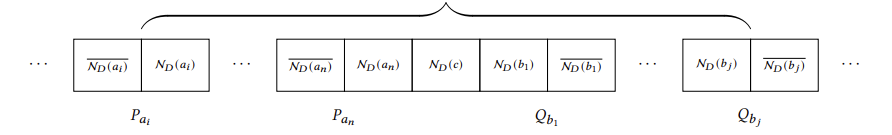
\includegraphics[width=1\linewidth]{Figure1.png}
    \caption{This figure depicts the range mode query corresponding to vertices $a_i, b_j$ and $c$. Here, $\mathcal{N}_D(v)$ denotes the set of neighbors of vertex $v$ in $D$, and $\overline{\mathcal{N}_D(v)}$ denotes the set of non-neighbors of vertex $v$ in $D$. }
    \label{fig:enter-label}
\end{figure}

\begin{multicols}{2}
    \textbf{Theorem 3.1} Assuming the $(2d+1)$-Clique hypothesis, there is no combinatorial data structure that solves Batch $d$-Dimensional  Orthogonal Range Mode in $O(n^{2-1/2d-\epsilon})$  time for $\epsilon > 0$.\\
    PROOF. We reduce from an unbalanced instance of $(2d+1)$-Clique Detection, where the first $2d$ parts $V_1, ..., V_{2d}$ all have sizes $n^{1/2d}$, while the last part $V_{2d+1}$ has size $n^{1-1/2d}$. By Fact, combinatorial algorithms for such unbalanced instances of $(2d+1)$-Clique Detection require $n^{2-1/2d-o(1)}$ time under the combinatorial $(2d+1)$-Clique hypothesis. 


For each $i \in [2d]$, we will first create an array $A_i$ of size $O(n)$ as follows. The elements in the array will be identified by vertices in $V_{2d+1}$. For each $v_i \in V_i$, we create a permutation of $V_{2d+1}$, such that the neighbors of $v_i$ in $V_{2d+1}$ appear before the non-neighbors of $v_i$ in $V_{2d+1}$. The array $A_i$ is then the concatenation of all the permutations. 

We can split each of the $d$ axes in $R^d$ at the origin to get a total of $2d$ half-axes. We will put each $A_i$ on one of the half-axes as follows. For each odd $i \in [2d]$ and each $j \in [|A_i|]$, we add a point whose $\lceil i/2 \rceil$-th coordinate is $j$ and whose other coordinates are all zeros. We assign a label $A_i[j]$ to this point. For each even $i \in [2d]$ and each $j \in [|A_i|]$, we add a point whose $\lceil i/2 \rceil$-th coordinate is $-j$ and whose other coordinates are all zeros. We similarly assign a label $A_i[j]$ to this point. 

Fix a tuple $(v_1, ..., v_{2d}) \in V_1 \times ... \times V_{2d}$. For every $i \in [2d]$, we use $b_i$ to denote the index in $A_i$ of the last neighbor of $v_i$ in the permutation corresponding to $\mathcal{N}_{V_{2d+1}}(v_i)$. Then we ask a range mode query on the orthogonal range defined as the following:\\
\begin{equation}
    \begin{cases}
       \ x_{\lceil(i/2)\rceil} \leq b_i :i\in [2d] & \text{is odd},\\ 
       x_{\lceil(i/2)\rceil} \geq -b_i  :i\in [2d] & \text{is even.} \nonumber 
    \end{cases}
\end{equation}


It is not hard to see that the multi-set of labels in this orthogonal range is exactly 
$$\{A_i[j]: 1 \leq i \leq 2d, 1 \leq j \leq b_i\}.$$
By construction of the arrays $A_i$, this multiset is the union of several full permutations of $V_{2d+1}$, and the neighborhoods of $v_1, ..., v_{2d}$ in $V_{2d+1}$. Thus, if $v_1, ..., v_{2d}$ have a common neighbor in $V_{2d+1}$, the  mode of the orthogonal range will also be a common neighbor. 

Therefore, by asking $O(n)$ range mode queries on this instance, we are able to determine whether each tuple $(v_1, ..., v_{2d}) \in V_1 \times \cdots \times V_{2d}$ has a common neighbor in $V_{2d+1}$, so that we can solve the $(2d+1)$-Clique Detection instance in $O(n)$ additional time. This concludes the lower bound proof for Batch $d$-Dimensional  Orthogonal Range Mode.


Similar to Dynamic Range Mode, the Batch $d$-Dimensional  Orthogonal Range Mode has a natural dynamic variant. 

\textbf{Proposition 3.2}\label{3.2}There is a combinatorial data structure that solves Dynamic d-Dimensional Orthogonal Range Mode in $O(n^{2-2/(2d+1)})$
pre-processing time, $O(n^{1-1/(2d+1)})$ query time and $O(n^{1-1/(2d+1)})$ update time.

\textbf{Theorem 3.3}\label{3.3}Assuming the combinatorial $(2d+2)$-Clique hypothesis, there is no combinatorial data structure that solves  Dynamic $d$-Dimensional  Orthogonal Range Mode in $(n)$ pre-processing time, $O(n^{1-1/(2d+1)-\epsilon})$ amortized query time and $O(n^{1-1/(2d+1)-\epsilon})$ amortized update time for $\epsilon > 0$.

\subsection{st Subgraph Connectivity}
\hline
\textbf{Algorithm 1}: the reduction from 4-Clique Detection to st-SubConn
\hline
\begin{enumerate}
    \item Initialize the st-SubConn data structure on G,letting S contain all vertices.
    \item  \textbf{for} $d \in D$ \textbf{do}
    \item \: \: \textbf{for} $a \in A$ \textbf{do}
    \item \: \: \:\: \: Let $a^{U_D} \in S$ if and only if $(a,d) \in E $.
    \item \:\:\: \: \textbf{for} $b \in B $ such that $(b,d) \in E$ \textbf{do}
    \item \: \:\:\:\:\: \: Let $b^{V_B} \in S.$
    \item \:\:\: \: \:\: \:\textbf{for} $ b'\in B/\{b\} $ \textbf{do}
    \item \:\:\: \: \:\: \:\: \: Let $(b')^{V_B} \notin S $
    \item  \:\:\: \: \:\: \:\textbf{for} $c \in C$ \textbf{do}
    \item  \:\:\:\: \:\: \:\: \:\: \:Let $c^{V_c} \in S$ if and only if $(c,d),(c,b) \in E$
    \item \:\:\: \: \:\: \: \textbf{if} s,t are connected in the induced subgraph of S\\ \textbf{then}
    \item \:\:\:\:\:\: \: \: \:\:\: \:\:\textbf{return} True
    \item \textbf{return} False
    
    
\end{enumerate}

\section{GEOMETRIC PROBLEMS AND OuMv$_k$
HYPOTHESIS}
\subsection{Skyline Points Counting}
\textbf{Proposition 4.4}\label{4.4} For any $k \ge 2$, there exists a data structure for Dynamic Skyline Points Counting in $R^{2k-1}$  in the semi-online model with $(n)$ pre-processing time and $(n^{1-1/k})$ update and query time. 

\textbf{ACKNOWLEDGMENTS}\\
We would like to thank Virginia Vassilevska Williams for many
helpful discussions during the early phase of this project. We also
thank her for valuable comments on a draft of this paper.

% \cite{abboud}
% \cite{7782962}
% \cite{DBLP:journals/corr/abs-1101-4068}
% \cite{elzein_et_al:LIPIcs.ESA.2018.25}
% \cite{inproceedings}
% \cite{doi:10.1137/090751670}
% \cite{doi:10.1137/S0097539702404389}
% \cite{6979028}
% \cite{10.1145/2746539.2746609}
\printbibliography

    
\end{multicols}




\end{document}
